\documentclass[a4paper,11pt,oneside]{memoir}
\chapterstyle{bianchi} %veelo, culver, crosshead, companion, bianchi

\usepackage{TUINFDA}

\usepackage{url}
\usepackage{hyperref}					% links in pdf
\usepackage{graphicx}            			% Figures
\usepackage{verbatim}            			% Code-Environment
\usepackage[lined,linesnumbered,algochapter]{algorithm2e} % Algorithm-Environment

\usepackage{pgf}					
\usepackage{tikz}					% tikz graphics
\usetikzlibrary{arrows,automata}

\usepackage{ngerman}
\usepackage[ngerman]{babel}
\usepackage{bibgerm,cite}       % Deutsche Bezeichnungen, Automatisches Zusammenfassen von Literaturstellen
\usepackage[ngerman]{varioref}  % Querverweise
% to use the german charset include cp850 for MS-DOS, ansinew for Windows and latin1 for Linux.
% \usepackage[latin1]{inputenc}

\usepackage{scrpage2}
\ifoot[]{}
\cfoot[]{}
\ofoot[\pagemark]{\pagemark}

\pagestyle{scrplain}



\thesistitle{Einsatz von ICT zur Steigerung der Energieeffizienz im landwirtschaftlichen Bereich}
\thesisdate{DD.MM.JJJJ}

\thesisdegree{Bachelor of Science(BSc)}{Bachelor of Science(BSc)}
\thesiscurriculum{Wirtschaftsinformatik}{Business Informatics} % your study
\thesisauthor{Martin Keiblinger} % your name
\thesismatrikelno{0825118} % your registration number

\thesisbetreins{Dipl.-Ing. Mag. Dr. Thomas Neubauer}

% define page numbering styles
\makepagestyle{numberCorner}
\makeevenfoot{numberCorner}{\thepage}{}{}
\makeoddfoot{numberCorner}{}{}{\thepage}

% define custom macros for specific formats or names
\newcommand{\uml}[1]{\texttt{#1}}
\newcommand{\cd}{\textsf{Class Diagram}}

\begin{document}

\captionnamefont{\bfseries}

%%%%%%%%%%%%%%%%%%%%%%%%%%%%%%%%%%%%%%%%%
%%%   FRONTMATTER    %%%%%%%%%%%%%%%%%%%%
%%%%%%%%%%%%%%%%%%%%%%%%%%%%%%%%%%%%%%%%%
\frontmatter
\pagenumbering{roman}

%%%%%%%%%%%%%%%%%%%%%%%%%%%%%%%%%%%%%%%%%
%%%   TITLEPAGES    %%%%%%%%%%%%%%%%%%%%%
%%%%%%%%%%%%%%%%%%%%%%%%%%%%%%%%%%%%%%%%%

% the german title page is required as first page
\selectlanguage{ngerman}

% setup page dimensions for titlepage
\newgeometry{left=2.4cm,right=2.4cm,bottom=2.5cm,top=2cm}

% force baselineskip and parindent
\newlength{\tmpbaselineskip}
\setlength{\tmpbaselineskip}{\baselineskip}
\setlength{\baselineskip}{13.6pt}
\newlength{\tmpparindent}
\setlength{\tmpparindent}{\parindent}
\setlength{\parindent}{17pt}

% first titlepage
\thispagestyle{tuinftitlepage}

%
% Kludge: for each titlepage set \pagenumbering to a different
% style. This is used to fix a problem with hyperref, because there
% are multiple "page 1" and hyperref hates that
%
\pagenumbering{Alph}

\begin{center}
{\ \vspace{4cm}}

\begin{minipage}[t][2.8cm][s]{\textwidth}%
\centering
\thesistitlefontHUGE\sffamily\bfseries\tuinfthesistitle\\
\bigskip
{\thesistitlefonthuge\sffamily\bfseries\tuinfthesissubtitle}
\end{minipage}

\vspace{4cm}

{\thesistitlefontLARGE\sffamily \tuinfthesistype}

\vspace{6mm}

{\thesistitlefontlarge\sffamily von}

\vspace{6mm}

{\thesistitlefontLarge\sffamily\bfseries \tuinfthesisauthor}

\vspace{1.5mm}

{\thesistitlefontlarge\sffamily Matrikelnummer \tuinfthesismatrikelno} 

\vspace{7cm}

\vspace{0pt}\raggedright\thesistitlefontnormalsize\sffamily


\begin{minipage}[t][1cm][t]{\textwidth}%
  \vspace{0pt}\raggedright\thesistitlefontnormalsize\sffamily
  %
  \begin{tabbing}%
	    \hspace{19mm} \= \hspace{66mm} \kill
	    \tuinfthesisbetreuung: \> \tuinfthesisbetreins
  \end{tabbing}
\end{minipage}

\begin{minipage}[t][1.5cm][t]{\textwidth}%
  \vspace{0pt}\sffamily\thesistitlefontnormalsize
  \begin{tabbing}%
    \hspace{35mm}  \kill
    Wien, \tuinfthesisdate  \\    \end{tabbing}
\end{minipage}

\end{center}

% we're done with the titlepages, proceed with default pagenumbering
\pagenumbering{roman}

% restore baselineskip
\setlength{\baselineskip}{\tmpbaselineskip}
\setlength{\parindent}{\tmpparindent}

% back to normal geometry
\restoregeometry

\newgeometry{left=2.5cm,right=2.5cm,bottom=2.5cm,top=2cm}

\selectlanguage{english}

%%% Local Variables:
%%% TeX-PDF-mode: t
%%% TeX-debug-bad-boxes: t
%%% TeX-parse-self: t
%%% TeX-auto-save: t
%%% reftex-plug-into-AUCTeX: t
%%% End:


%%%%%%%%%%%%%%%%%%%%%%%%%%%%%%%%%%%%%%%%%
%%%   ERKLAERUNG DER SELBSTAENDIGKEIT   %
%%%%%%%%%%%%%%%%%%%%%%%%%%%%%%%%%%%%%%%%%

\selectlanguage{ngerman}
\chapter*{Erklärung zur Verfassung der Arbeit}

\tuinfthesisauthor\\
\tuinfthesisauthoraddress

\vspace*{1.2cm}

Hiermit erkläre ich, dass ich diese Arbeit selbständig verfasst habe, 
dass ich die verwendeten Quellen und Hilfsmittel vollständig angegeben 
habe und dass ich die Stellen der Arbeit - einschließlich Tabellen, 
Karten und Abbildungen -, die anderen Werken oder dem Internet im 
Wortlaut oder dem Sinn nach entnommen sind, auf jeden Fall unter Angabe 
der Quelle als Entlehnung kenntlich gemacht habe.\\

\vspace*{2cm}
\begin{tabbing}%
    \hspace{58mm} \= \hspace{28mm} \= \hspace{58mm} \kill
    {\raggedright\rule{58mm}{0.5pt}} \> \> {\raggedright\rule{58mm}{0.5pt}} \\
    \begin{minipage}[t][0.5cm][t]{58mm}
	\vspace{0pt}\sffamily\thesistitlefontnormalsize
	\centering (Ort, Datum)
    \end{minipage}
    \> \>
    \begin{minipage}[t][0.5cm][t]{58mm}
	\vspace{0pt}\sffamily\thesistitlefontnormalsize
	\centering (Unterschrift \tuinfthesisverfassung)
    \end{minipage}
\end{tabbing}


\selectlanguage{english}

%%%%%%%%%%%%%%%%%%%%%%%%%%%%%%%%%%%%%%%%%
%%%   ABSTARCT    %%%%%%%%%%%%%%%%%%%%%%%
%%%%%%%%%%%%%%%%%%%%%%%%%%%%%%%%%%%%%%%%%

\chapter*{Abstract}

Energy efficiency in agriculture is as important as never before. The industrial countries have to work under massive cost pressure whereas developing countries have to compensate their scarcity of resources like watter or electrical energy. The purpose of this work is to give an overview of the the most important research topics for this matter.

The approach for was to find papers which are about the most important research topics defined by the agenda for transnational co-operation on energy efficiency in agriculture of the EU. 

As result this paper shows a survey of papers for mathematical optimization models, sensor network technology, GIS-systems, artificial intelligence and planning systems like decision support systems. The essence of this work is the presentation suitable solutions for optimizing processes and resource consumption. 



%%%%%%%%%%%%%%%%%%%%%%%%%%%%%%%%%%%%%%%%%
%%%   CONTENTS    %%%%%%%%%%%%%%%%%%%%%%%
%%%%%%%%%%%%%%%%%%%%%%%%%%%%%%%%%%%%%%%%%
% uncomment to set document language to german (results in "Inhaltsverzeichnis", "Kapitel", "Abbildung", etc. instead of "Contents", "Chapter", and "Figure"), otherwise the document's language is english
%\selectlanguage{ngerman}

\setcounter{tocdepth}{1}

\cleardoublepage
\pagestyle{numberCorner}
\tableofcontents*

%%%%%%%%%%%%%%%%%%%%%%%%%%%%%%%%%%%%%%%%%
%%%   MAINMATTER    %%%%%%%%%%%%%%%%%%%%%
%%%%%%%%%%%%%%%%%%%%%%%%%%%%%%%%%%%%%%%%%

\mainmatter
\pagenumbering{arabic}
\pagestyle{numberCorner}

%%%%%%%%%%%%%%%%%%%%%%%%%%%%%%%%%%%%%%%%%
\chapter{Introduction}
\label{ch:intro}
%%%%%%%%%%%%%%%%%%%%%%%%%%%%%%%%%%%%%%%%%

\section{Motivation}

Landwirtschaft spielt für jede Gesellschaft eine entscheidende Rolle, da ohne sie die Ernährung der Bürger unmöglich wäre. Für einen Staat ist eine moderne und effiziente Landwirtschaft wichtig um Abhängigkeiten zu anderen Staaten zu verhindern oder zumindest zu verringern. Daher ist dieses Thema auch für Länder der ersten Welt nach wie vor auf der Agenda. Da die Personalkosten hoch sind, ist die Effizenzsteigerung durch Technologie entscheidend für die Entwicklung des Landwirtschaftssektor.

Durch den ständig steigenden Energiebedarf ist vor allem die Frage nach eines optimalen Einsatzes von Energie wichtig für Zukunft der Landwirtschaftsbetriebe in der EU. Neben der Forschung in den Disziplinen der Chemie und des Maschinenbaus, ist die Informatik eine interessante Quelle für kleine und große Optimierungen des landwirtschaftlichen Betriebs. Da ich den Blick über den Tellerrand nicht nur nicht scheue sondern gerne wage und selbst aus einem landwirtschaftlich genutzten Gebiet in Niederösterreich, dem Marchfeld, stamme, liegt mir die Zukunft der Landwirtschaft in Europa am Herzen.

\section{Problemstellung}

Diese Arbeit beschäftigt sich mit der Ausarbeitung des aktuellen Standes der Steigerung der Energieeffizenz in der Landwirtschaft mittels Informations- und Kommunikationstechnik, kurz ICT. Dazu wird eine Zusammenfassung der aktuellen Forschungsprojekte in der EU erstellt und dann eine Zusammenfassung der für Effizenzsteigerung durch ICTs relevanten Literatur erstellt. Dabei wird Wert auf die Ausarbeitung der Forschungsschwerpunkte und Auflistung der für Vergleiche nötigen Kennzahlen. 

Ziel ist es eine Übersicht der relevanten Literatur für folgende Arbeiten zu erstellen.

\section{Verwendete Methode}

Die Quellen für diese Arbeit wurden ohne Fokus auf bestimmte Konfernzen oder Datenbanken ausgewählt. Es wurden alle Arbeiten und Projekte die zumindest innerhalb der EU eine Rolle spielen ausgewertet.

\subsection{Literaturrecherche}
Um möglichst keine relevanten Arbeiten zu übersehen wurden neben den akademischen Datenbanken und Bibliotheken auch Berichte von relevanten Forschungsgruppen der EU herangezogen. Die dort erwähnten Projekte und Arbeiten wurden dann gezielt weiter verfolgt. Für die Suche nach Literatur wurden verschiedene Kombinationen aus folgenden Suchbegriffen gewählt:

\textit{energy, efficency, it, informatic, stochastic, agriculture, Landwirtschaft, Effizenz, ICT, Informationstechnologie, Planung}

\subsection{Selektionsvorgang}
Die wissenschaftliche Literatur wurde auf Basis folgender Kriterien bewertet:
\begin{itemize}
  \item ICT-Relevanz. Bei der Suche nach Effizenz in der Landwirtschaft mussten alle Themen aussortiert werden die sich auf Effizenzsteigerung durch chemische Präparate oder bestimmte Entwicklungen im Maschinenbau bezogen.
  \item Veröffentlichungsmedium. Arbeiten die weder im Rahmen einer Konfernz noch in einem Journals oder zumindestens in einem wissenschaftlichen Magazins veröffentlicht wurden, wurden aussortiert.
  \item Aktualität. Die Arbeiten mussten relativ aktuell sein. Werke die vor 2010 geschrieben wurden, wurden nicht weiter verfolgt.
\end{itemize}

Neben wissenschaftlicher Literatur sind auch Reports von aktuellen Forschungsprojekte eine wichtige Quelle. Bei diesen Projekten wurde ebenfalls auf Aktualität geachtet.

\section{Verwandte Arbeiten}
Eine Übersicht der verschiedenen Forschungsrichtungen wird im Bericht des Projekts D4.5 Agenda for Transnational Co-operation on energy efficency in agriculture geboten.\cite{misc:Mikkola2013}.


%%%%%%%%%%%%%%%%%%%%%%%%%%%%%%%%%%%%%%%%%

\section{General Information}

This document is intended as a template and guideline and should support the author in the course of doing the bachelor's thesis.
Assessment criteria comprise the quality of the theoretical and/or practical work as well as structure, content and wording of the written bachelor's thesis. Careful attention should be given to the basics of scientific work (e.g., correct citation).

\section{Structure of the Thesis}

The table of contents is followed by the introduction and the main part, which can vary according to the content. The bachelor's thesis ends with the bibliography (compulsory) and the appendix (optional).

\begin{itemize}
  \item	Cover page
  \item Acknowledgements
  \item Abstract of the thesis in English and German
  \item Table of contents
  \item Introduction (5-10\%)
  	\begin{itemize}
  		\item motivation
  		\item problem statement (which problem should be solved?)
  		\item aim of the work
  		\item methodological approach
  		\item structure of the work
  	\end{itemize}
  \item State of the art / analysis of existing approaches (10-30\%)
  	\begin{itemize}
  		\item literature studies
  		\item analysis
  		\item comparison and summary of existing approaches
  	\end{itemize}
  \item Suggested solution/Implementation/Methodology (20-50\%)
  	\begin{itemize}
  		\item used concepts
  		\item methods and/or models
  		\item languages
  		\item design methods
  		\item data models
  		\item analysis methods
  		\item formalisms
  	\end{itemize}
  \item Critical reflection (10-20\%)
  	\begin{itemize}
  		\item comparison with related work
  		\item discussion of open issues
  	\end{itemize}
  \item Summary and future work (5\%)
  \item Appendix: source code, data models, \dots
  \item Bibliography
\end{itemize}


\section{Recommendations}

\begin{itemize}
	\item Use primary literature, i.e., cite the original work.
	\item Refer diverse source of literature.
	\item Use active language (e.g., 'The programmer prepared a test plan and distributed it to the team' instead of 'A test plan was prepared and distributed to the team by the programmer'). 
	\item Cite all figures and tables in the text (e.g., Fig. 1 shows ...).
	\item Cite figures in the caption.
	\item Redraw cited figures.
	\item Use a spell checker (TexnicCenter => Extras => Options).
	\item Proof read the thesis several times. Let other people proof read your work.
	
	
\end{itemize}



 



%%%%%%%%%%%%%%%%%%%%%%%%%%%%%%%%%%%%%%%%%
\chapter{Typographic Design}
\label{ch:typo}
%%%%%%%%%%%%%%%%%%%%%%%%%%%%%%%%%%%%%%%%%


For working with LaTeX you can take advantage of a variety of books and free introductions and tutorials on the internet. A competent contact point for LaTeX beginners is the LaTeX Wikibook, which is available under \url{http://en.wikibooks.org/wiki/LaTeX}. 

Recommended clients for working with LaTeX are TexnicCenter \url{http://www.toolscenter.org}. TexnicCenter demands Miktext as prerequisite \url{http://prdownloads.sourceforge.net/miktex}.



The following sections give examples of the most important LaTeX environments and commands.

\section{Tables}

Tables have to be realized with the help of the \textit{table} environment. Tables shall be sequentially numbered for each chapter and described in terms of a short caption (cf. Table~\ref{tab:diplomaseminar}).

\begin{table}[htb]
	\centering
	\begin{tabular}{|l|c|c|}
		\hline \textbf{Name} & \textbf{Date} & \textbf{Title} \\
		\hline
		\hline Mustermann Adam  & 18.5   & T1    \\
		\hline Musterfrau Eva  & 22.6   & T2    \\
		\hline
	\end{tabular}
	\caption{Seminar for Master Students}
	\label{tab:diplomaseminar}
\end{table}


\section{Figures}

Like tables, figures shall be sequentially numbered for each chapter and described in terms of a short caption). You could either produce your drawings directly inside Latex using PSTricks\footnote{\url{http://tug.org/PSTricks}}, Tikz\footnote{\url{http://sourceforge.net/projects/pgf}}, or any set of macros dedicated to your requirements (cf. Figure~\ref{fig:samplefigure_tikz}). Alternatively, you may include figures prepared in external tools (cf. Figure~\ref{fig:samplefigure_pdf}). Note, to ensure high quality printing, all figures must have at least 300 dpi.

\begin{figure}
	\centering
	\begin{tikzpicture}[->, auto, node distance=2.8cm, semithick]
	  \node[initial, state] (1)		 {$S_1$};
	  \node[state] 		(2) [right of=1] {$S_2$};
	
	  \path (1) edge [bend left]  node {0} (2)
		(1) edge [loop above] node {1} (1)
		(2) edge [bend left]  node {0} (1)
		(2) edge [loop above] node {1} (2);
	\end{tikzpicture}
	\caption{Sample figure}
	\label{fig:samplefigure_tikz}
\end{figure}

\begin{figure}[tb]
	\centering
	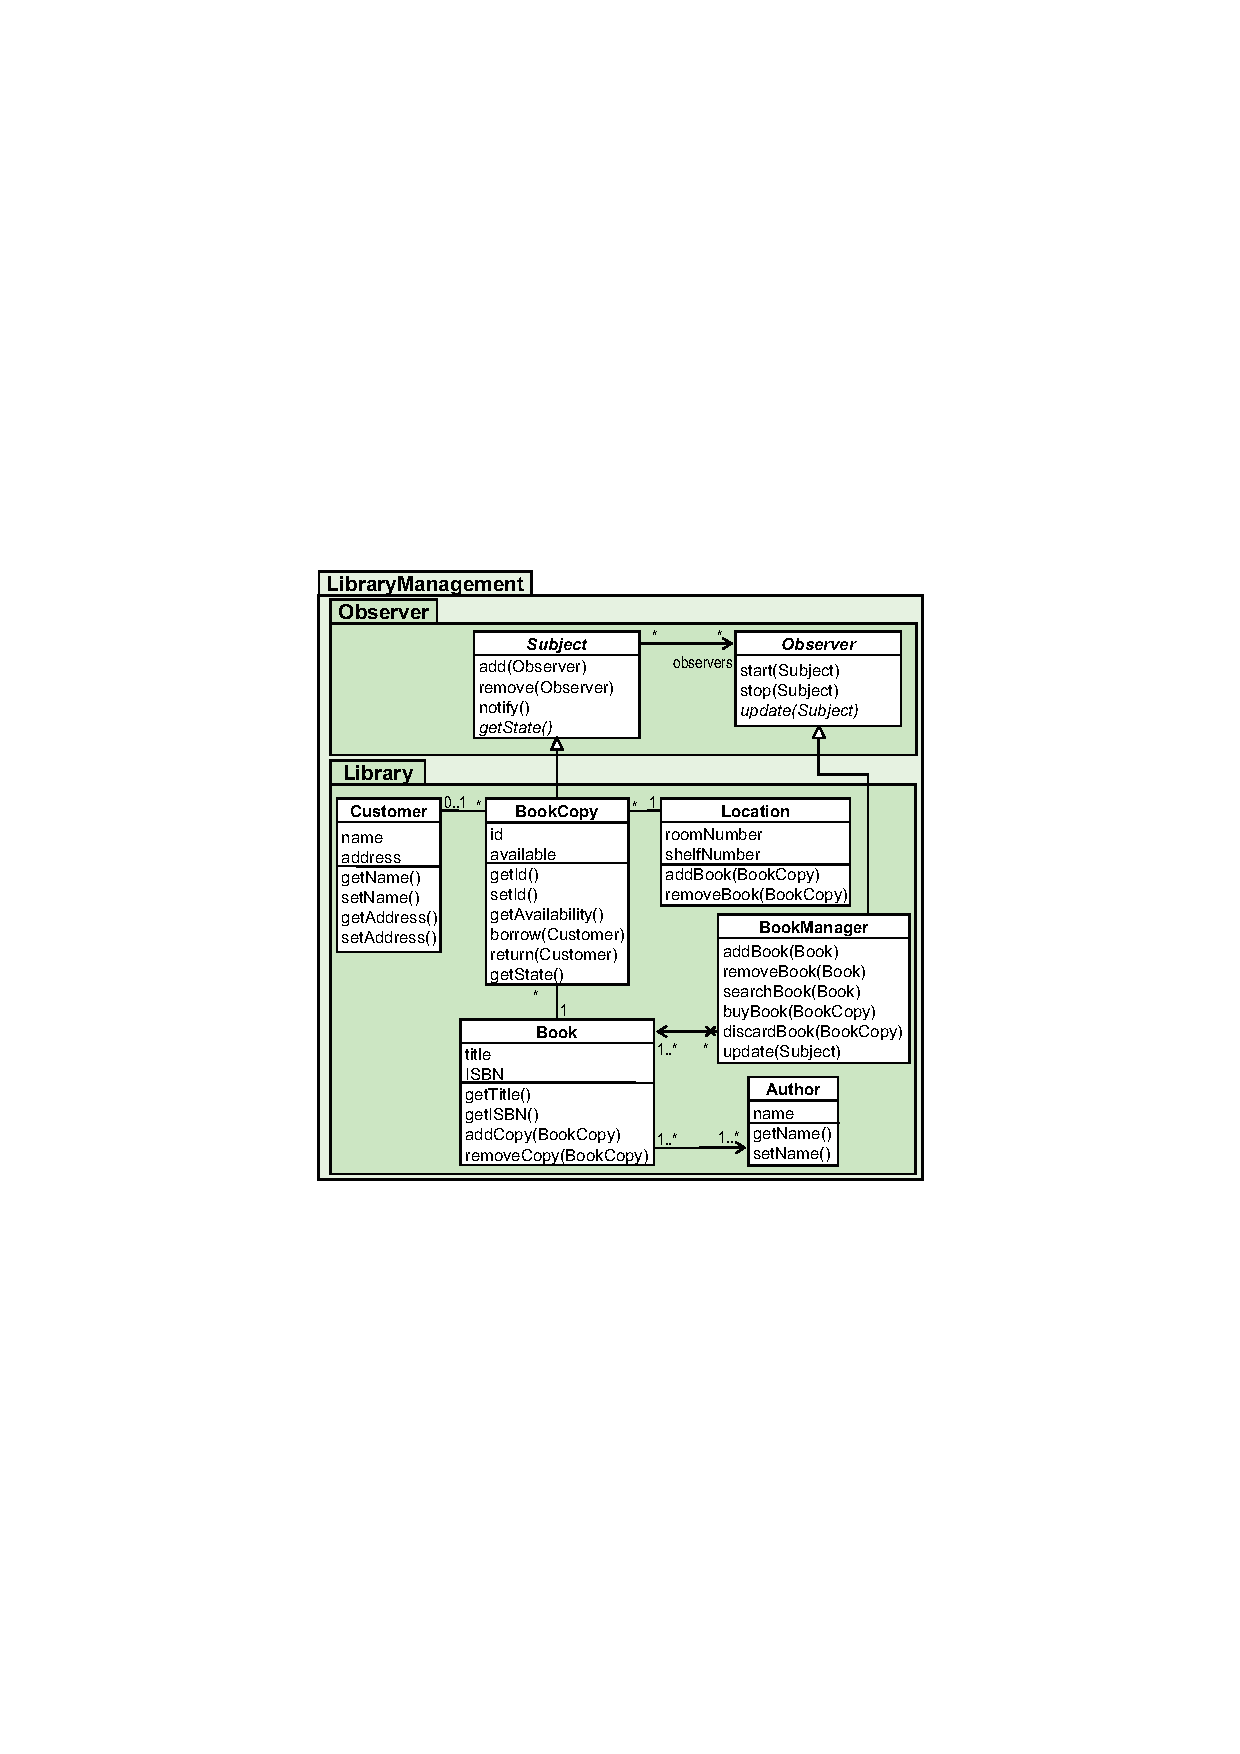
\includegraphics[width=0.7\textwidth]{figures/figure1}
	\caption{Sample figure}
	\label{fig:samplefigure_pdf}
\end{figure}


\section{Fonts}

When introducing important terms for the first time use \emph{emphasize}. For a consistent look and feel of proper names like {\cd} and {\uml{Observer}} pattern you may define macros in the main document \texttt{thesis.tex}.

\section{Code}

For short code fragments use the \textit{verbatim} environment.

\begin{verbatim}
//Start Program
System.out.println("Hello World!");
//End Program
\end{verbatim}

A much better alternative is the \textit{algorithm} environment (cf. Algorithm~\ref{alg:samplealgorithm}). This environment offers special formatting features for loops, operations and comments.

\begin{algorithm}[t]
\SetKwData{Left}{left}
\SetKwData{This}{this}
\SetKwData{Up}{up}
\SetKwFunction{Union}{Union}
\SetKwFunction{FindCompress}{FindCompress}
\SetKwInOut{Input}{input}
\SetKwInOut{Output}{output}

\Input{A bitmap $Im$ of size $w\times l$}
\Output{A partition of the bitmap}

\BlankLine

\emph{special treatment of the first line}\;
\For{$i\leftarrow 2$ \KwTo $l$}{
\emph{special treatment of the first element of line $i$}\;
\For{$j\leftarrow 2$ \KwTo $w$}{\label{forins}
\Left$\leftarrow$ \FindCompress{$Im[i,j-1]$}\;
\Up$\leftarrow$ \FindCompress{$Im[i-1,]$}\;
\This$\leftarrow$ \FindCompress{$Im[i,j]$}\;
\If(\tcp*[r]{O(\Left,\This)==1}){\Left compatible with \This}{\label{lt}
\lIf{\Left $<$ \This}{\Union{\Left,\This}}\;
\lElse{\Union{\This,\Left}\;}
}
\If(\tcp*[r]{O(\Up,\This)==1}){\Up compatible with \This}{\label{ut}
\lIf{\Up $<$ \This}{\Union{\Up,\This}}\;
\tcp{\This is put under \Up to keep tree as flat as possible}\label{cmt}
\lElse{\Union{\This,\Up}}\tcp*[r]{\This linked to \Up}\label{lelse}
}
}
\lForEach{element $e$ of the line $i$}{\FindCompress{p}}
}
\caption{Sample algorithm}\label{alg:samplealgorithm}
\end{algorithm}



%%%%%%%%%%%%%%%%%%%%%%%%%%%%%%%%%%%%%%%%%
\chapter{Bibliographic Issues}
\label{ch:bibliographic}
%%%%%%%%%%%%%%%%%%%%%%%%%%%%%%%%%%%%%%%%%

\section{Literature Search}


\section{BibTeX}

BibTeX should be used for referencing. JabRef (an open source tool for Windows) is recommended for the management of references. 

The LaTeX source document of this pdf document provides you with different samples for references to journals~\cite{jour:B2BServices}, conference papers~\cite{proc:TheWebMLApproach}, books~\cite{book:umlatwork}, book chapters~\cite{incoll:ErhardKonrad1992}, electronic standards~\cite{man:BPEL}, dissertations~\cite{phdthesis:manuelWimmer}, masters' theses~\cite{mast:AUMLProfile}, and web sites~\cite{misc:BIGWebsite}. The respective BibTeX entries may be found in the file \texttt{references.bib}. For administration of the BibTeX references we recommend \url{http://www.citeulike.org} or JabRef for offline administration, respectively.


%%%%%%%%%%%%%%%%%%%%%%%%%%%%%%%%%%%%%%%%%
%%% BACKMATTER %%%%%%%%%%%%%%%%%%%%%%%%%%
%%%%%%%%%%%%%%%%%%%%%%%%%%%%%%%%%%%%%%%%%

\appendix

\bibliographystyle{plain}
\bibliography{references}

\end{document}
